%!TEX root = ../Thesis.tex

\chapter{Workshop 2}
\label{appendix:workshop2}
\lhead{}
De workshop begon met een uitleg van de concepten die behandeld gaan worden waarna de niet-programmeurs zelfstandig de opdrachten gingen maken.

Er is voor elke deelnemer een test omgevingen aangemaakt waar de VRInteractions plugin geïnstalleerd is en een aantal voorbeelden bevat die als hulp gebruikt kunnen worden.

\section{Doel}
\begin{itemize}
	\item Kennis laten maken met de VRInteractions plugin en een tv aan en uit zetten door er naar te kijken.
	\item Door de deelnemers zelf te laten programmeren en daardoor het doel van de komende workshops te laten bepalen. 
\end{itemize}

\section{Opdrachten}

\subsection{Opdracht 1}
Zet de TV aan door er naar te kijken en pauzeer hem als er niet meer naar gekeken wordt.

In het oefenproject staat een TV met een promo video van DPI. 
Voeg de LookEvents component aan de TV blueprint toe.
Koppel vervolgens de play en pause van de media texture, het filmpje, aan de Lookevents door middel van de LookEvents component.

\subsection{Opdracht 2}
Zorg dat de LookEvents makkelijker getriggerd worden door een Collisie box te laten bepalen wanneer er naar de TV gekeken wordt.

Voeg een collison box toe aan de tv blueprint en zet zijn collisie profile op custom en zet alle collisie op ignore behalve de visibility. De visibility moet namelijk op overlap.

Creëer een begin play event en sleep de LookEvents Component in de blueprint. Als je op van de exit node een lijn sleept en los laat kan je in het pop up window zoeken naar “Set Seen Trigger”. Hiermee geef je aan dat je de events wil laten afvuren als naar een specifiek component van de blueprint gekeken wordt. Zet vervolgens de gemaakte Box Collision als de trigger parameter.

\subsection{Opdracht 3}
Stel de LookEvents in zodat de TV op een kortere (of langere) afstand getriggerd wordt.

Als je de look events component in het components venster (links boven) selecteert verschijnt er aan de rechter kant in het details venster de instelling hiervan. 
Verander de waardes onder de kopjes “User Interaction” en “Trigger” totdat jij tevreden bent met het resultaat.

\subsection{Opdracht 4}
Maak een loader die het kijken naar het object duidelijk maakt.

Voeg een statische mesh component toe en zet de statische mesh op de standaard materialshpere.
In de tick functie van de blueprint vraag je de “Seen Progress” van de lookevents door de functie “Get Seen Progress” Op de lookevents component aan te spreken.
Creëer nu een “Lerp(Vector”) door met een rechte muisknop in de blueprints het zoek venster te opennen en hierin te zoeken naar de functie.
Zet als waarde A de begin locatie van de Loader en als waarde B zijn eind waarde (waar hij naartoe gaat bewegen)
Vervolgens pak zet je relative locatie  van de loader op de return value van de lerp.

\section{Resultaten}
Uiteindelijk zijn de deelnemers samen de opdracht gaan maken en hebben het volgende ingeleverd:

Yo Mark,

We hebben dit even gezamenlijk gedaan. 

Hier wat onduidelijk heden.

Opdracht 1: we konden in eerste instantie de play node niet vinden.
Het was wat onduidelijk dat we de movie texture moesten verslepen naar media player target.

Opdracht 2 en 3: Event begin play was niet duidelijk. Deze triggerde het filmpje vanaf het begin.
zoals in de afbeelding te zien.

\begin{figure}[!ht]
  \centering
    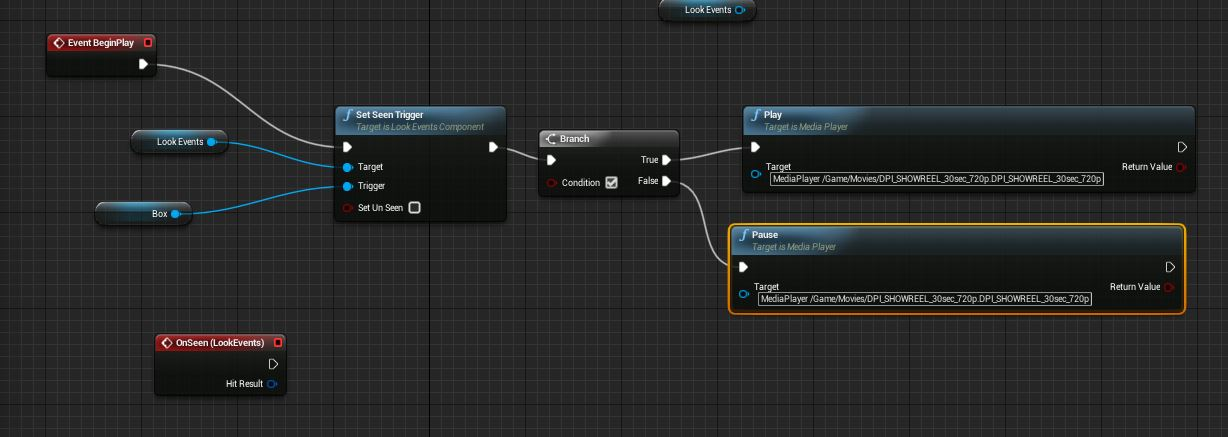
\includegraphics[width=\linewidth,height=\textheight,keepaspectratio]{Workshop_2_Opdracht23_fout}
    \caption{Niet werkende Blueprint van opdracht twee en drie.}
\end{figure}

We probeerde ook wat uit met Branch, maar helaas.

Daarna hebben we weer alles vastgekoppeld aan de OnSeen look event en aan de Event beginPlay. Dit bleek wel te werken.

\begin{figure}[!ht]
  \centering
    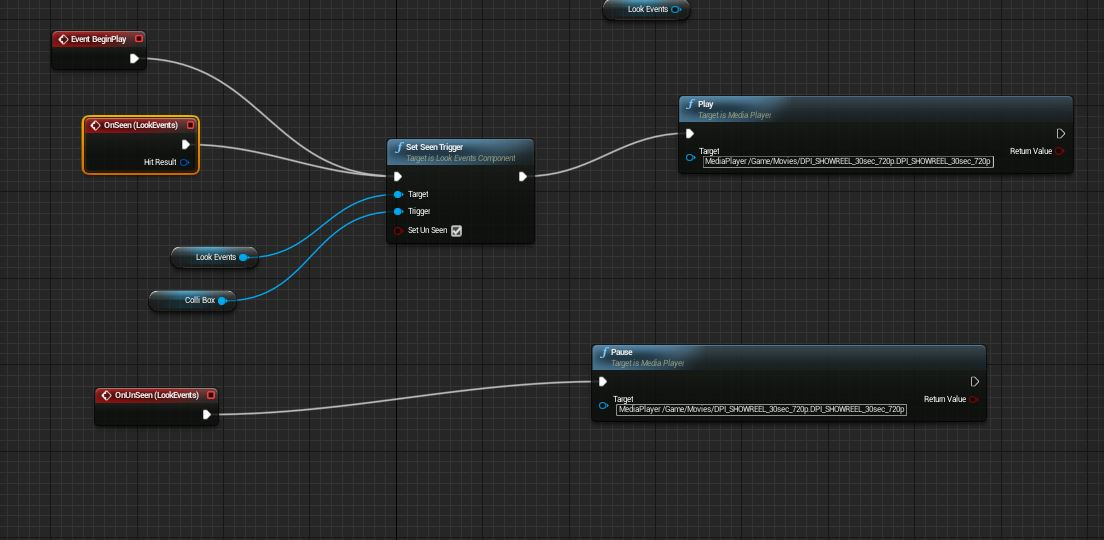
\includegraphics[width=\linewidth,height=\textheight,keepaspectratio]{Workshop_2_Opdracht23_werkend}
    \caption{Functionele Blueprint van opdracht twee en drie.}
\end{figure}


Opdracht4: Uitleg was beter, plaatje werkte ook mee, maar op zich allemaal logisch.

\begin{figure}[!ht]
  \centering
    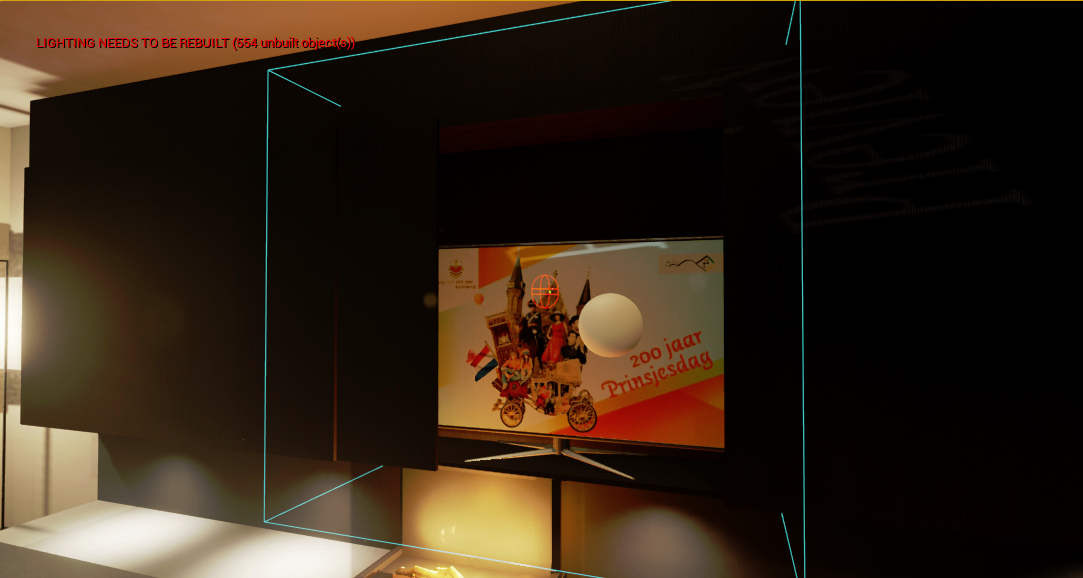
\includegraphics[width=\linewidth,height=\textheight,keepaspectratio]{Workshop_2_eindresultaat}
    \caption{Eind resultaat van de opdrachten.}
\end{figure}

\section{Reflectie}
Het probleem van de play node vinden was inderdaad lastig omdat dit een uitzondering is op hoe de rest van \gls{ue4} werkt. De enige manier om dit soort problemen op te lossen is door ervaring krijgen met hoe de {ue4} werkt.

De uitwerking van opdracht twee en drie was werkend maar het zetten van de LookEvents optie werd in het Tick event gedaan wat voor onverwachte functionaliteit kan zorgen. Dit had eigenlijk tijdens de Begin Play moeten gebeuren.

Na het bespreken van de opdrachten is er gezamenlijk gekozen om de volgende workshops op dezelfde manier aan te pakken; uitleg en dan zelfstandige opdrachten. Ook is er besloten om langzaam dieper in Blueprint scripting te duiken.

